\documentclass[brazil]{beamer}
\usepackage{pacotesLaTeX}

\title{Cadeia de Ising com campo transverso}
\author{Thales Freitas Macêdo}  

\begin{document}

\frame{\titlepage}

\begin{frame}{Modelo de Ising clássico}
    O modelo de Ising é um modelo de spins \( S_i = \pm 1 \) localizados, formando uma rede, sob ação de um campo magnético externo \( H \), alinhado com os spins.
    \[ E = - J \sum_{\expval{ij}} S_i S_j - \mu H \sum_i S_i \]
\end{frame}

\begin{frame}{Cadeia de Ising com campo transverso}
    O modelo de Ising com campo transverso é obtido ao impor que a direção do campo magnético seja transversa à direção dos spins.
    Agora, não podemos mais tratar o problema classicamente, e temos que usar a mecânica quântica.
    Vou abordar o problema unidimensional da cadeia de Ising.
    \begin{equation}
        H = - \sum_i \qty[\Gamma S_i^x + J S_i^z S_{i + 1}^z] = - \sum_i \qty[S_i^x + \lambda S_i^z S_{i + 1}^z] \label{hamiltoniano}
    \end{equation}
    onde \( S^\alpha \) é o operador de spin de Pauli na direção \( \alpha \), \( J \) é a constante de interação entre os spins, \( \Gamma \) é a constante do campo, e \( \lambda = J / \Gamma \), com \( \Gamma = 1 \).
\end{frame}

\begin{frame}{Cadeia de Ising com campo transverso}
    Definimos o gap de massa \( \Delta (\lambda) \) como a diferença de energia entre o estado fundamental e o primeiro estado excitado.
    Numa transição de fase quântica, \( \Delta = 0 \), e o comprimento de correlação \( \xi = 1 / \Delta \) diverge.
\end{frame}

\begin{frame}{Método \textit{Finite-Size Scaling}}
    Nesse método, diagonalizamos exatamente o Hamiltoniano para cadeias com \( N = 2, 3, 4, \dots \) spins.
    A princípio, uma cadeia com muitos spins aproximaria o limite termodinâmico \( N \to \infty \) mais adequadamente, mas pode ser numericamente muito custoso.
    Podemos usar a seguinte relação para estimar os parâmetros no limite termodinâmico:
    \begin{equation}
        \lambda_c (L) = \lambda_c + A L^{-1/\nu} ,
    \end{equation}
    onde \( \lambda_c \) é valor crítico de \( \lambda \) para uma transição de fase quântica, \( L \) representa os tamanhos das cadeias, \( A \) é uma constante e \( \nu \) é um expoente crítico relacionado ao comprimento de correlação \( \xi \).
\end{frame}

\begin{frame}{Método \textit{Finite-Size Scaling}}
    Na base de autovalores de \( S^x \), as representações matriciais de \( S^\alpha \) para o espaço de 1 spin são
    \begin{equation}
        S^x = \mqty(
        1 & 0 \\
        0 & -1
        )
    \end{equation}
    e
    \begin{equation}
        S^z = \mqty(
        0 & 1 \\
        1 & 0
        ) .
    \end{equation}
    Temos agora que obter uma representação matricial dos operadores \( S_i^\alpha \).
\end{frame}

\begin{frame}{Método \textit{Finite-Size Scaling}}
    No espaço de estados de \( N \) spins, temos que fazer o produto tensorial entre \( S_i^\alpha \) e operadores identidade para os outros spins.
    A representação do produto tensorial desses operadores é obtido pelo produto de Kronecker:
    \begin{equation}
        \vb{A} \otimes \vb{B} = \mqty(
        a_{11} \vb{B} & \dots & a_{1n} \vb{B} \\
        \vdots & \ddots & \vdots \\
        a_{m1} \vb{B} & \dots & a_{mn} \vb{B}
        )
    \end{equation}
\end{frame}

\begin{frame}{Método \textit{Finite-Size Scaling}}
    Por exemplo, se \( N = 4 \):
    \begin{equation}
        H = - \qty(S_1^x + S_2^x + S_3^x + S_4^x) - \lambda (S_1^z S_2^z + S_2^z S_3^z + S_3^z S_4^z) .
    \end{equation}
    Para estabelecer condições de contorno periódicas, basta adicionar o termo \( - \lambda S_4^z S_1^z \).
\end{frame}

\begin{frame}{Método \textit{Finite-Size Scaling}}
    Encontrei o gap de massa para os casos \( N = 2, 3, 4, 5, 6, 7, 8, 9, 10 \):
    \begin{figure}
        \centering
        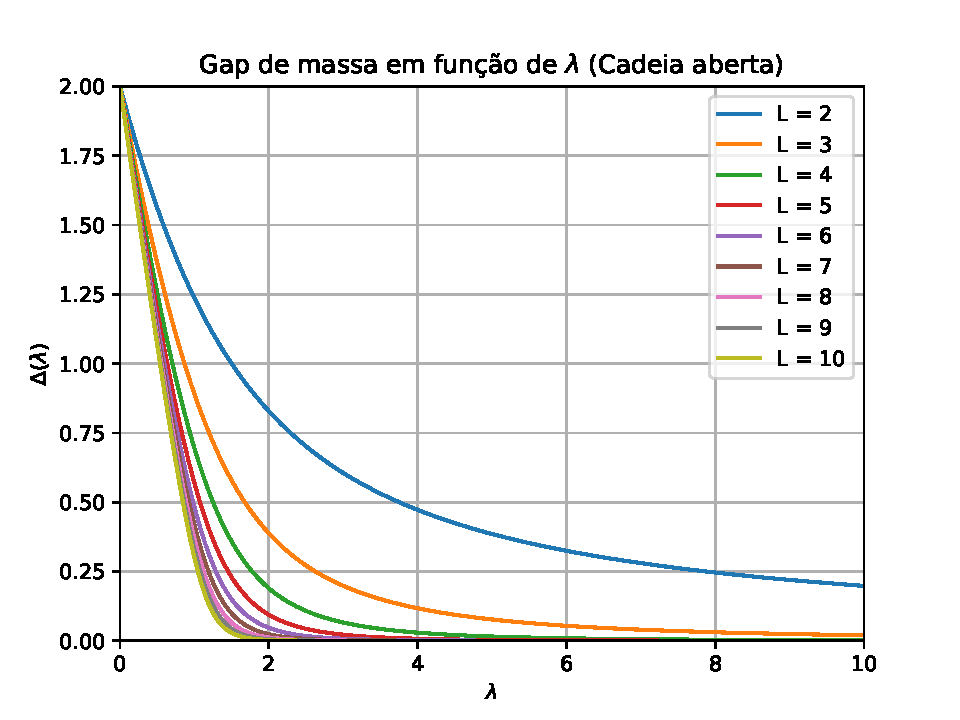
\includegraphics[width=0.7\textwidth]{gap.pdf}
    \end{figure}
\end{frame}

\begin{frame}{Método \textit{Finite-Size Scaling}}
    Encontrei o gap de massa para os casos \( N = 2, 3, 4, 5, 6, 7, 8, 9, 10 \):
    \begin{figure}
        \centering
        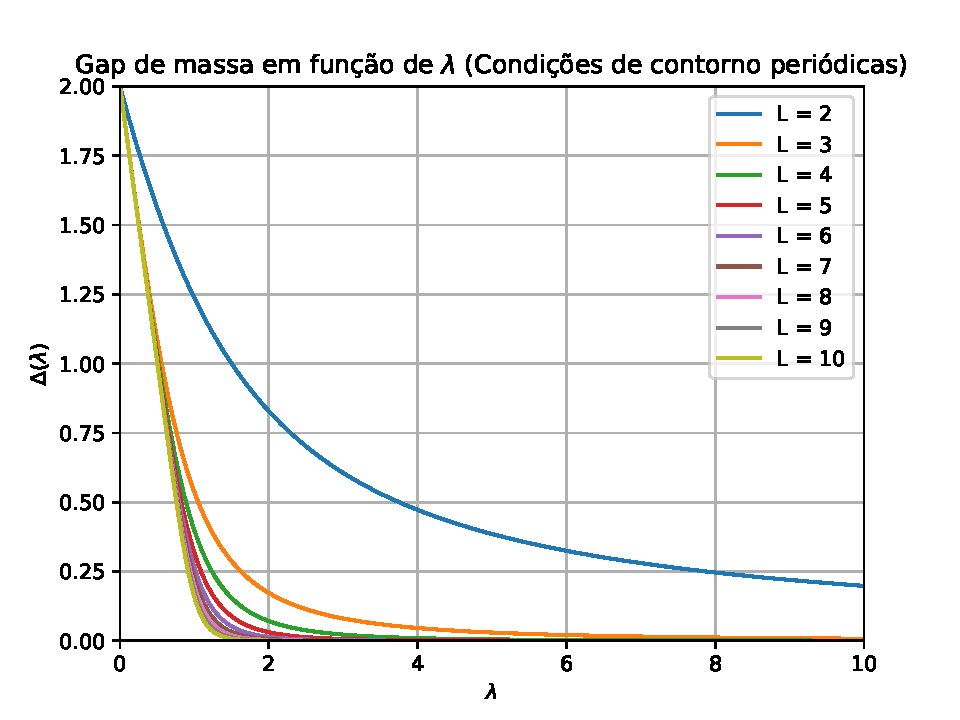
\includegraphics[width=0.7\textwidth]{gap_ccp.pdf}
    \end{figure}
\end{frame}

\begin{frame}{Método \textit{Finite-Size Scaling}}
    Os gaps de massa tendem a zero no infinito para cadeias finitas.
    Só há transição de fase quântica no limite termodinâmico.
    Temos que estimar de alguma forma \( \lambda_c \) para os casos finitos.
    Uso a razão de gap de massa:
    \begin{equation}
        R_L = \frac{L \Delta(\lambda, L)}{(L - 1) \Delta (\lambda, L - 1)} .
    \end{equation}
    O parâmetro crítico \( \lambda_c \) pode ser aproximado como a solução da equação \( R_L (\lambda_c) = 1 \).
\end{frame}

\begin{frame}{Método \textit{Finite-Size Scaling}}
    Calculei os \( \lambda_c \) e plotei em função de \( L \):
    \begin{figure}
        \centering
        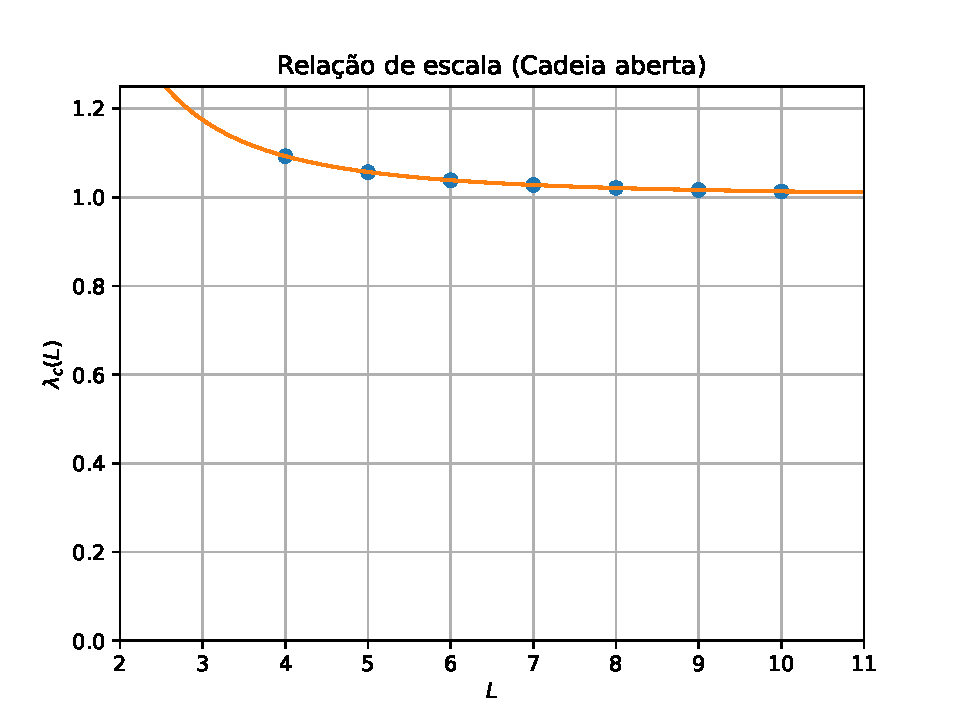
\includegraphics[width=0.7\textwidth]{rel_escala.pdf}
    \end{figure}
    O ajuste à função \( f(x) = c + A x^k \) forneceu
    \begin{align*}
        c = \num{1.0013(2)} &  & A = \num{1.98(3)} &  & k = \num{-2.22(1)}
    \end{align*}
\end{frame}

\begin{frame}{Método \textit{Finite-Size Scaling}}
    Calculei os \( \lambda_c \) e plotei em função de \( L \):
    \begin{figure}
        \centering
        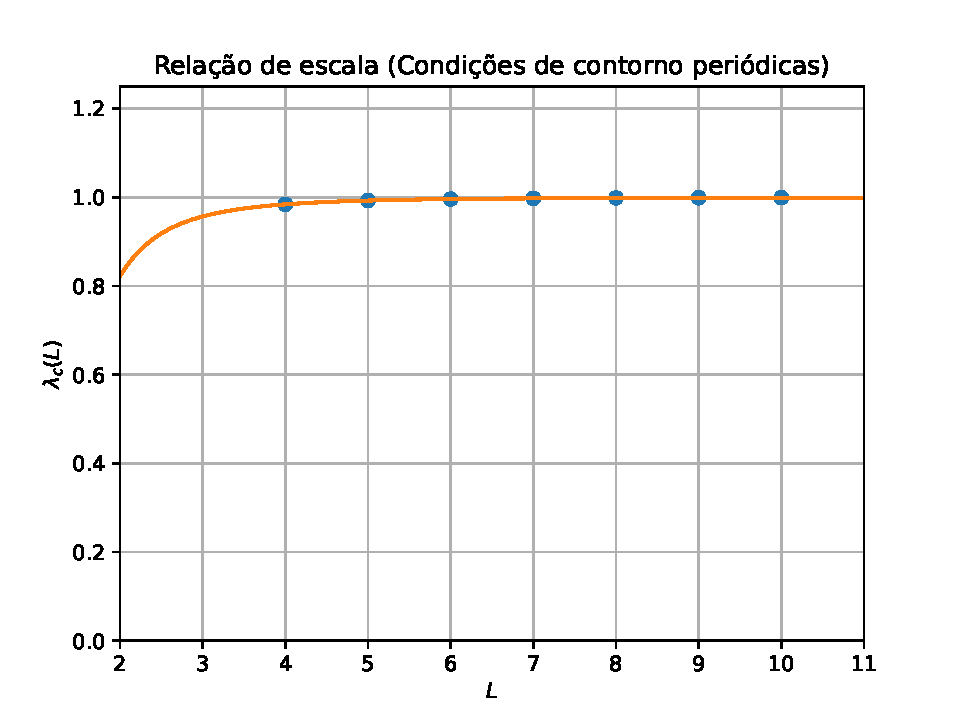
\includegraphics[width=0.7\textwidth]{rel_escala_ccp.pdf}
    \end{figure}
    O ajuste à função \( f(x) = c + A x^k \) forneceu
    \begin{align*}
        c = \num{0.99984(3)} &  & A = \num{-2.01(5)} &  & k = \num{-3.50(2)}
    \end{align*}
\end{frame}

\begin{frame}{Método \textit{Block Renormalisation Group}}
    Os valores críticos do problema da cadeia de Ising transversa tem como propriedade ser invariante de escala: ou seja, alterar a escala do problema não altera o ponto crítico. O método iterativo \textit{Block Renormalisation Group} altera a escala do problema em busca dos pontos críticos, que são os pontos fixos após as iterações.

    O método consiste em um procedimento que produza o Hamiltoniano (\ref{hamiltoniano}) na \( n \)-ésima iteração:
    \begin{equation}
        H^{(n)} = - \sum_i \qty( J^{(n)} S_i^{x (n)} S_{i + 1}^{x (n)} + h^{(n)} S_i^{z (n)} ) + C^{(n)} \sum_i I_i^{(n)} , \label{H_n}
    \end{equation}
    com as condições iniciais \( J^{(0)} = J \), \( h^{(0)} = h \) e \( C^{(0)} = 0 \), e onde \( I_i^{(n)} \) indica a matriz identidade \( 2 \times 2 \) para o spin no sítio \( i \).
\end{frame}

\begin{frame}{Método \textit{Block Renormalisation Group}}
    Para a \( n \)-ésima iteração, dividimos a cadeia em blocos com \( n_s \) spins em cada bloco.
    Usando os índices \( j \) para indicar o bloco, e \( p \) para indicar o spin dentro do bloco, reescrevemos o hamiltoniano sob a forma
    \begin{equation}
        H^{(n)} = \sum_j \qty( H_j^{(n)} + H_{j, j + 1}^{(n)} + C^{(n)} \sum_{p = 1, \dotsc , n_s} I_{j, p}^{(n)} ) , \label{H_j}
    \end{equation}
    onde \( H_j^{(n)} \) é o Hamiltoniano intra-bloco:
    \begin{equation}
        H_j^{(n)} = - J^{(n)} \sum_{p = 1, \dotsc, n_s - 1} S_{j, p}^{x(n)} S_{j, p + 1}^{x(n)} - h^{(n)} \sum_{p = 1, \dotsc, n_s} S_{j, p}^{z(n)}
    \end{equation}
    e \( H_{j, j + 1}^{(n)} \) é o Hamiltoniano inter-bloco:
    \begin{equation}
        H_{j, j + 1}^{(n)} = - J^{(n)} S_{j, n_s}^{x(n)} S_{j + 1, 1}^{x(n)}
    \end{equation}
\end{frame}

\begin{frame}{Método \textit{Block Renormalisation Group}}
    Por exemplo, para uma cadeia de 4 spins e um bloco de 2 spins,
    \begin{align}
        H^{(0)} = & - J^{(0)} \qty( S_1^x S_2^x + S_2^x S_3^x + S_3^x S_4^x ) \\
                  & - h^{(0)} \qty( S_1^z + S_2^z + S_3^z + S_4^z )           \\
        =         & - J^{(0)} S_1^x S_2^x - h^{(0)} ( S_1^z + S_2^z )         \\
                  & - J^{(0)} S_3^x S_4^x - h^{(0)} ( S_3^z + S_4^z )         \\
                  & - J^{(0)} S_2^x S_3^x
    \end{align}
    onde podemos ver os termos intra-bloco e inter-bloco.
\end{frame}

\begin{frame}{Método \textit{Block Renormalisation Group}}
    Agora diagonalizamos o Hamiltoniano \( H_j^{(n)} \) no espaço de estados do bloco gerado pela base de kets
    \begin{equation}
        \ket{\epsilon_1, \epsilon_2, \dotsc, \epsilon_p, \dotsc, \epsilon_{n_s}} ,
    \end{equation}
    com \( \epsilon_p = \pm 1 \) correspondendo aos autoestados de \( S_{j, p}^{z(n)} \).

    Somente usamos os estados fundamental \( \ket{+}^{(n + 1)} \) e primeiro excitado \( \ket{-}^{(n + 1)} \), de energias \( E_+^{(n + 1)} \) e \( E_-^{(n + 1)} \), respectivamente:
    \begin{gather}
        \ket{+}^{(n + 1)} = \sum^+ \lambda_{\epsilon_1, \epsilon_2, \dotsc, \epsilon_p, \dotsc, \epsilon_{n_s}}^{+ (n)} \ket{\epsilon_1, \epsilon_2, \dotsc, \epsilon_p, \dotsc, \epsilon_{n_s}} , \\
        \ket{-}^{(n + 1)} = \sum^- \lambda_{\epsilon_1, \epsilon_2, \dotsc, \epsilon_p, \dotsc, \epsilon_{n_s}}^{- (n)} \ket{\epsilon_1, \epsilon_2, \dotsc, \epsilon_p, \dotsc, \epsilon_{n_s}}.
    \end{gather}
\end{frame}

\begin{frame}{Método \textit{Block Renormalisation Group}}
    Introduzimos um novo conjunto de operadores de spin \( S_j^{x (n + 1)} \) associados ao bloco \( j \), tal que os autoestados de \( S_j^{z (n + 1)} \) sejam \( \ket{+}^{(n + 1)} \) e \( \ket{-}^{(n + 1)} \).
    Assim, podemos reescrever \( H_j^{(n)} \) na forma renormalizada
    \begin{equation}
        H_j^{(n)} = - h^{(n + 1)} S_j^{z (n + 1)} + \frac{1}{2} \qty( E_+^{(n + 1)} + E_-^{(n + 1)} ) I_j^{(1)} , \label{intrabloco}
    \end{equation}
    onde
    \begin{equation}
        h^{(n + 1)} = \frac{1}{2} \qty(E_-^{(n + 1)} - E_+^{(n + 1)}) . % \qc c^{(1)} = \frac{E_1 + E_0}{2} .
    \end{equation}
\end{frame}

\begin{frame}{Método \textit{Block Renormalisation Group}}
    Tomando os elementos de matriz do operador anterior \( S_{j, p}^{x (n)} \) entre os estados \( \ket{+}^{(n + 1)} \) e \( \ket{-}^{(n + 1)} \), obtemos a relação de recursão de spins
    \begin{equation}
        S_{j, p}^{x (n)} = \xi_p^{x(n)} S_j^{x(n + 1)} ,
    \end{equation}
    com
    \begin{equation}
        \xi_p^{x(n)} = \mel{+}{S_{j, p}^{x (n)}}{-} = \sum^+ \lambda_{\epsilon_1, \dotsc, \epsilon_p, \dotsc, \epsilon_{n_s}}^{+ (n)} \lambda_{\epsilon_1, \dotsc, - \epsilon_p, \dotsc, \epsilon_{n_s}}^{- (n)}.
    \end{equation}
    Assim podemos reescrever \( H_{j, j + 1}^{(n)} \) em termos dos novos operadores de spin:
    \begin{equation}
        H_{j, j + 1}^{(n)} = - J^{(n + 1)} S_j^{x(n + 1)} S_{j + 1}^{x(n + 1)} \label{interbloco}
    \end{equation}
    com \( J^{(n + 1)} = \qty( \xi_1^{x(n)} )^2 J^{(n)} \) .
\end{frame}

\begin{frame}{Método \textit{Block Renormalisation Group}}
    Ao colocar os termos (\ref{intrabloco}) e (\ref{interbloco}) no Hamiltoniano (\ref{H_j}), reobtemos um Hamiltoniano com a mesma forma de (\ref{H_n}) para o iteração \( n + 1 \), com nova constante
    \begin{equation}
        C^{(n + 1)} = n_s C^{(n)} + \frac{1}{2} \qty( E_+^{(n + 1)} + E_-^{(n + 1)} ) .
    \end{equation}
    Com essa constante, podemos calcular a energia por sítio do estado fundamental, dada pela relação
    \begin{equation}
        (E_0 / N)_{N \to \infty} = \lim_{n \to \infty} \qty(C^{(n)} / n_s^n) ,
    \end{equation}
    e assim podemos calcular a susceptibilidade magnética no eixo \( z \) pela relação
    \begin{equation}
        \chi_z = - \dv[2]{h} (E_0 / N) .
    \end{equation}
\end{frame}

\begin{frame}{Método \textit{Block Renormalisation Group}}
    \framesubtitle{NumPy/ SciPy}
    \begin{figure}
        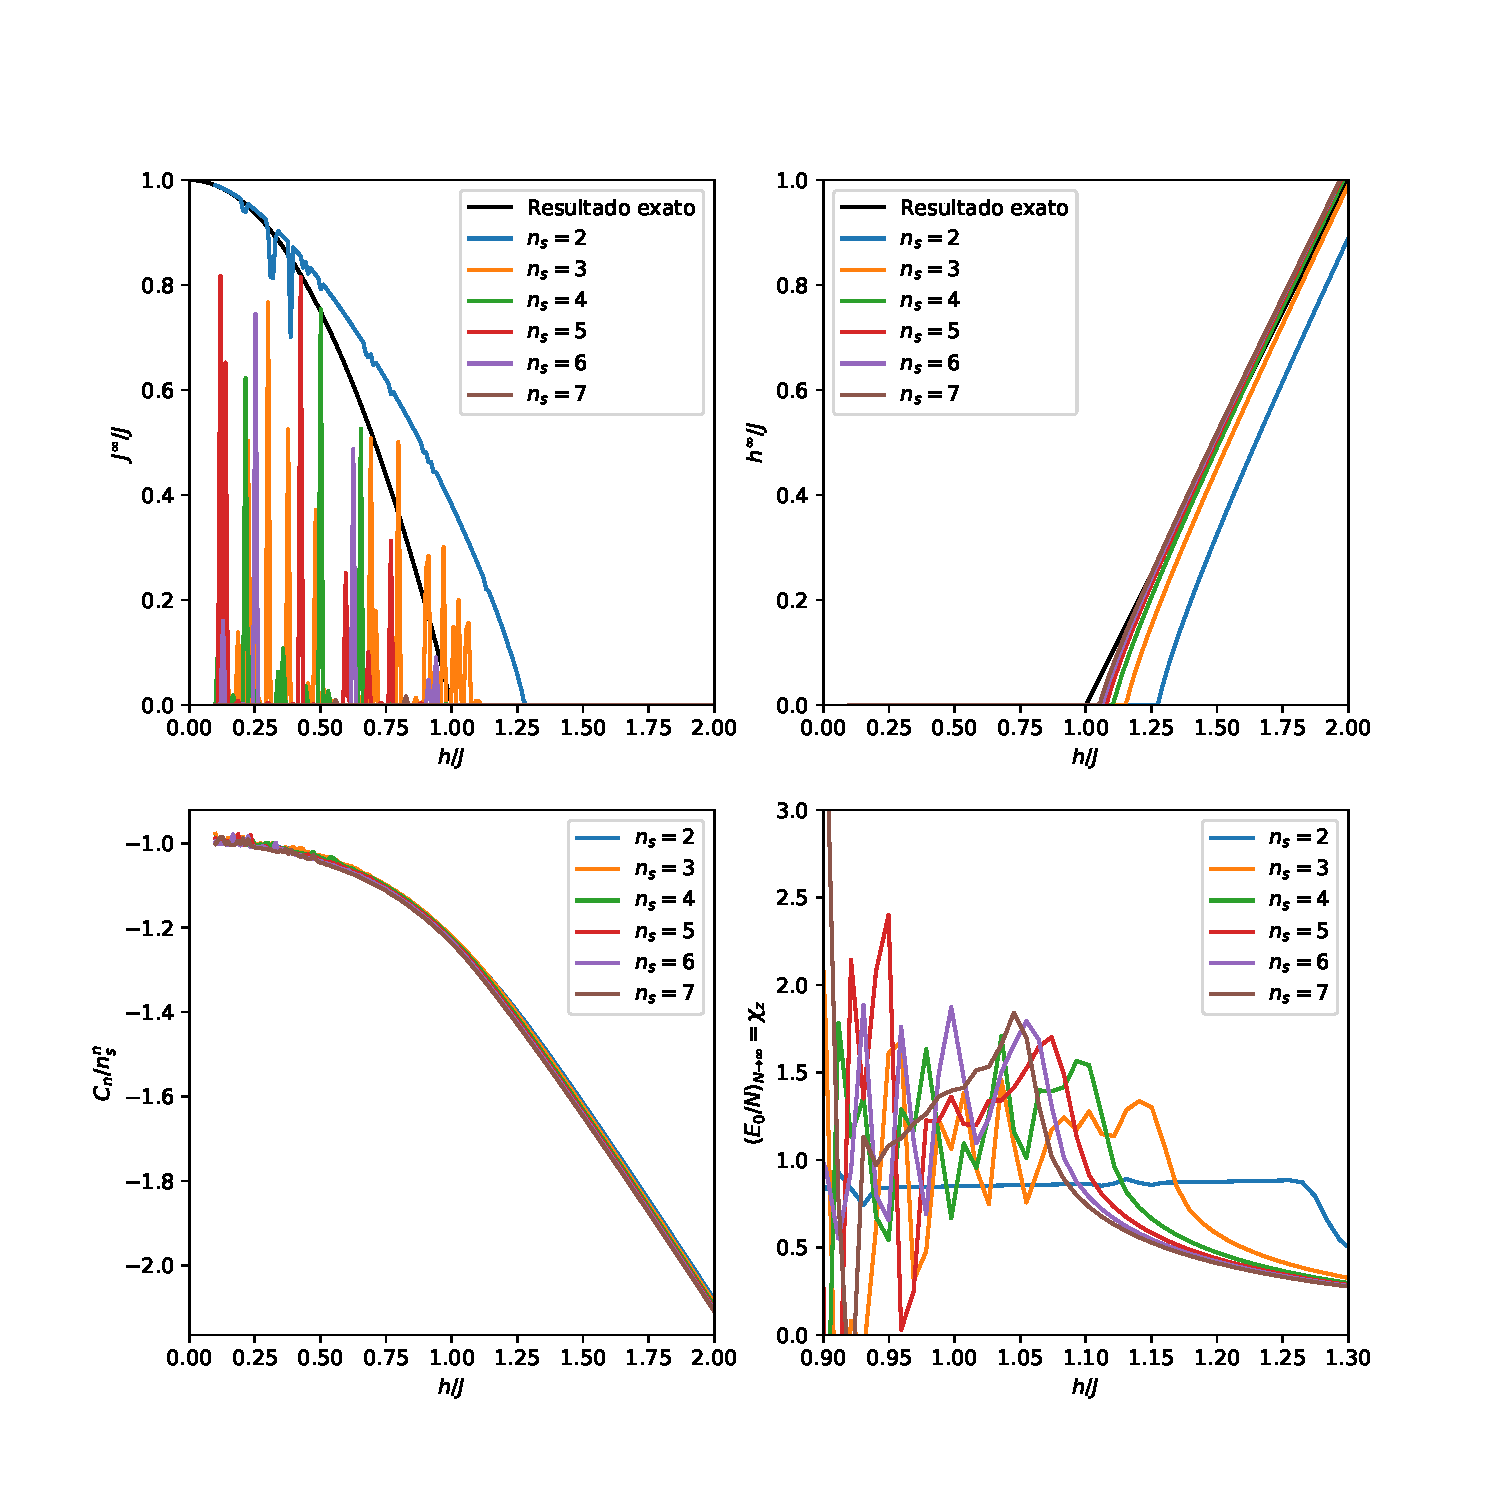
\includegraphics[width=0.73\textwidth]{teste_numpy.pdf}
    \end{figure}
\end{frame}

\begin{frame}{Método \textit{Block Renormalisation Group}}
    \framesubtitle{mpmath}
    \begin{figure}
        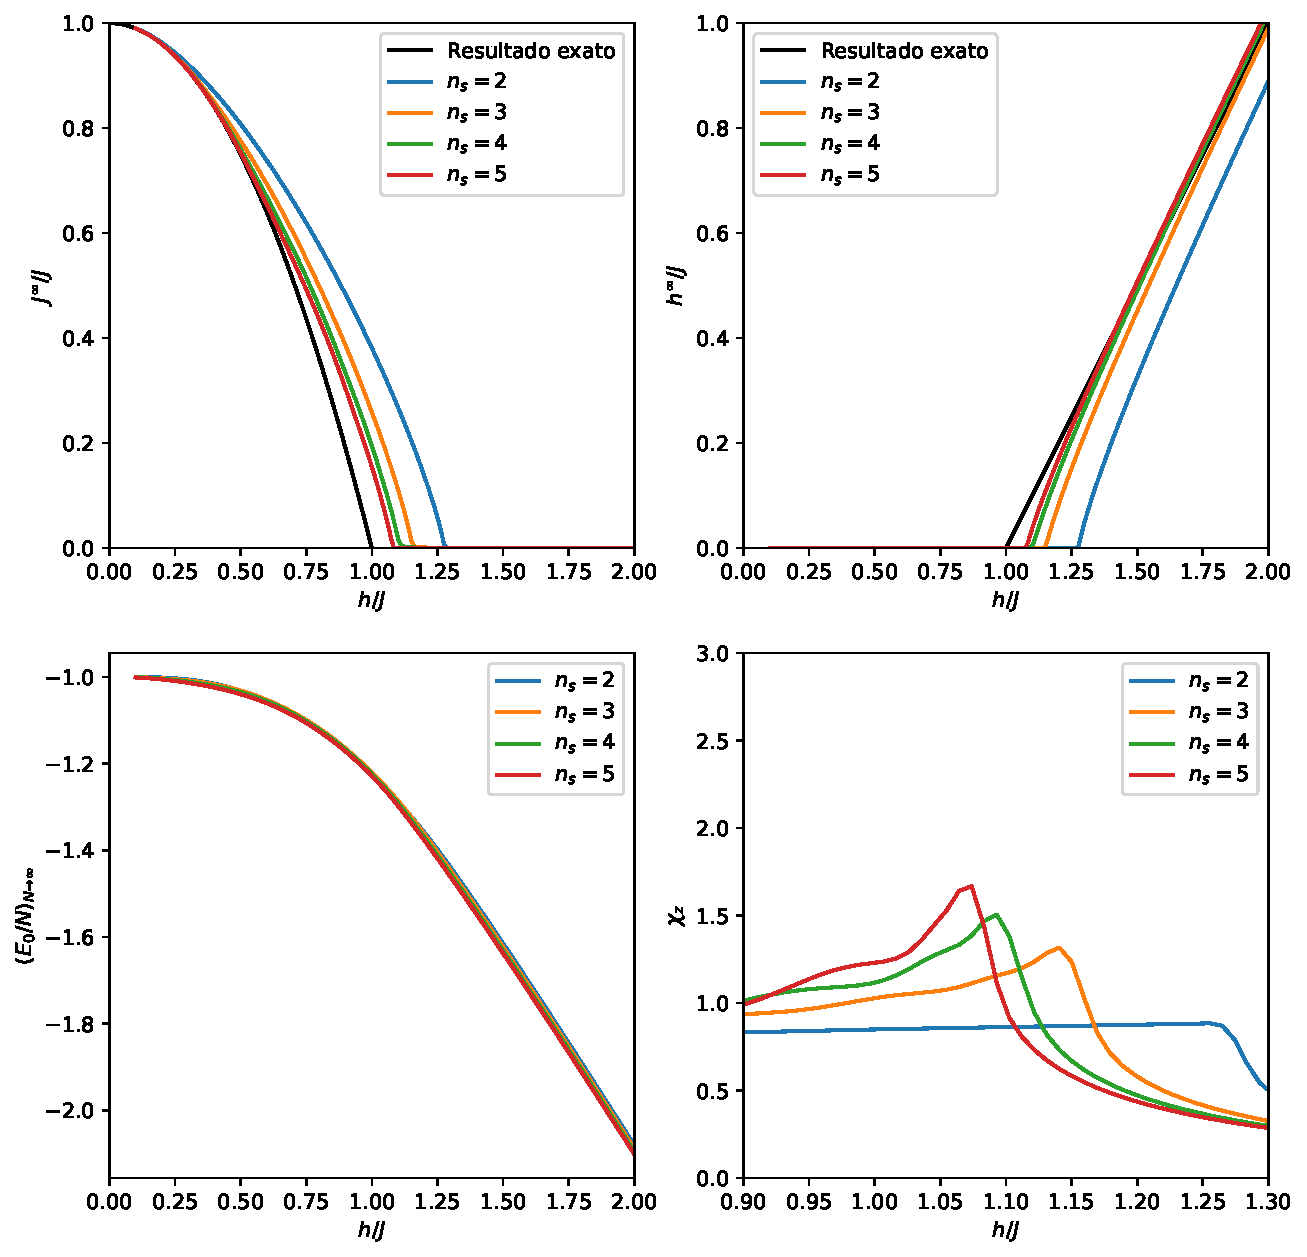
\includegraphics[width=0.73\textwidth]{renorm.pdf}
    \end{figure}
\end{frame}

\begin{frame}
    \frametitle{Referências}
    \nocite{*}
    \bibliographystyle{plain}
    % \bibliographystyle{amsalpha}
    \bibliography{refs}
\end{frame}

% \bibliography{refs} % Entries are in the refs.bib file

\end{document}
